\item 27.4-9

A - nicotine

B - kerosene

C - water

Assume dilute and that kerosene and water are perfectly imiscible.

\begin{align*}
    & V_{N+1} = 100 \\
    & y_{A,N+1} = 0.014 \\ 
    & y_{B,N+1} = 0.986 \\ 
    V' &= V_{N+1} \left(1 - y_{B,N+1}\right) = 100 \cdot \left(1 - 0.986\right) \\
    V' &= 98.6 \\
    \intertext{90\% removal of nicotine}
    x_{A,N} L_N &= 0.9 \cdot 1.4 \\
    y_{A,1} V_1 &= 0.1 \cdot 1.4 \\
    y_{B,1} V_1 &= 98.6 \\
    \intertext{Solve $V_1$ mass balance}
    y_{A,1} &= 0.00142 \\
    \intertext{Organic inlet and aqueous outlet are in equilibrium.}
    \intertext{From equilibrium data in Example 27.4-3, at $y_{A,N+1}=0.014$}
    x_{A,N} &= 0.015 \\
    \intertext{Mass balance for $L'_{\text{min}}$}
    L'_{\text{min}} \frac{x_0}{1-x_0} + V' \frac{y_{N+1}}{1-y_{N+1}} &= L'_{\text{min}} \frac{x_N}{1-x_N} + V' \frac{y_1}{1-y_1} \\
    L'_{\text{min}} \frac{0}{1-0} + 98.6 \cdot \frac{0.014}{1-0.014} &= L'_{\text{min}} \frac{0.015}{1-0.015} + 98.6 \cdot \frac{0.00148}{1-0.00148} \\
    L'_{\text{min}} &= 81.8 \text{ kg/h} \\
    L' &= 1.5 L'_{\text{min}} \\
    L' &= 122.7 \text{ kg/h} \\
    \intertext{From mass balance at L'}
    x_0 &= 0 \\
    y_{N+1} &= 0.014 \\
    x_N &= 0.0102 \\
    y_1 &= 0.00142 \\
    \intertext{Assume dilute and a straight operating line.}
    \intertext{Plot operating and equilibrium line at step off stages.}
\end{align*}

\begin{center}
    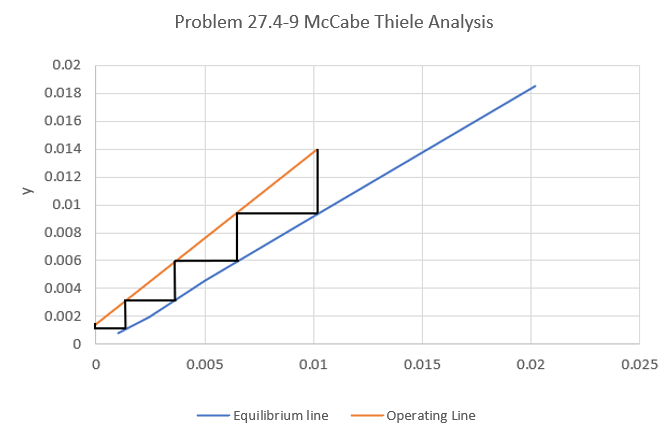
\includegraphics[width=0.8\textwidth]{assets/p3.png}
\end{center}

Last stage does not fully reach operating line. $\boxed{N\approx3.8}$